\section{The Unit Step Function}

\noindent
In the next section we'll consider initial value problems
$$
ay''+by'+cy=f(t),\quad y(0)=k_0,\quad y'(0)=k_1,
$$
where $a$, $b$, and $c$ are constants and $f$ is  piecewise continuous.
 In this section we'll develop procedures for using the
table of Laplace transforms to find  Laplace transforms of
piecewise continuous functions, and to find the piecewise continuous
inverses of Laplace transforms.

\begin{example}\label{example:8.4.1}\rm
 Use the table of Laplace transforms to find the Laplace
transform of
\begin{equation} \label{eq:8.4.1}
f(t)=\left\{\begin{array}{cl}
2t+1,&0\le t<2,\\[1\jot]
 3t,&t\ge2
\end{array}\right.
\end{equation}
(Figure~\ref{figure:8.4.1}).
\end{example}

\solution Since the formula for $f$ changes at $t=2$, we write
\begin{equation}\label{eq:8.4.2}
\begin{array}{ccl}
{\cal L}(f)&=&\dst \int_0^\infty e^{-st}f(t)\,dt\\[2\jot]
&=&\dst\int_0^2 e^{-st}(2t+1)\,dt+\int_2^\infty e^{-st}(3t)\,dt.
\end{array}
\end{equation}
To relate the first term to a Laplace transform,  we   add and subtract
$$
\int_2^\infty e^{-st}(2t+1)\,dt
$$
in \eqref{eq:8.4.2} to obtain
\begin{equation}\label{eq:8.4.3}
\begin{array}{ccl}
{\cal L}(f)&=&\dst\int_0^\infty e^{-st}(2t+1)\,dt+
\int_2^\infty e^{-st}(3t-2t-1)\,dt\\[2\jot]
&=&\dst\int_0^\infty e^{-st}(2t+1)\,dt+
\int_2^\infty e^{-st}(t-1)\,dt\\[2\jot]
&=&\dst{\cal L}(2t+1)+\int_2^\infty e^{-st}(t-1)\,dt.
\end{array}
\end{equation}
To relate  the last integral to a Laplace transform,
  we make the change of variable
 $x=t-2$   and rewrite the integral as
\begin{eqnarray*}
\int_2^\infty e^{-st}(t-1)\,dt&=&\int_0^\infty e^{-s(x+2)}(x+1)\,dx
\\[2\jot]
&=&e^{-2s}\int_0^\infty e^{-sx}(x+1)\,dx.
\end{eqnarray*}
Since the symbol used for the variable of integration has no effect on the
value of a definite integral, we can now replace $x$ by the more standard
$t$ and write
$$
\int_2^\infty e^{-st}(t-1)\,dt
=e^{-2s}\int_0^\infty e^{-st}(t+1)\,dt=e^{-2s}{\cal L}(t+1).
$$
This and \eqref{eq:8.4.3} imply that
$$
{\cal L}(f)={\cal L}(2t+1)+e^{-2s}{\cal L} (t+1).
$$
Now we can use the table of Laplace transforms to find that
$$
{\cal L}(f)={2\over s^2}+{1\over s} +e^{-2s}\left({1\over s^2}+{1\over
s}\right).\bbox
$$

\begin{figure}[H]
\color{blue}
  \begin{minipage}[b]{0.5\linewidth}
    \centering
   \scalebox{.65}{
  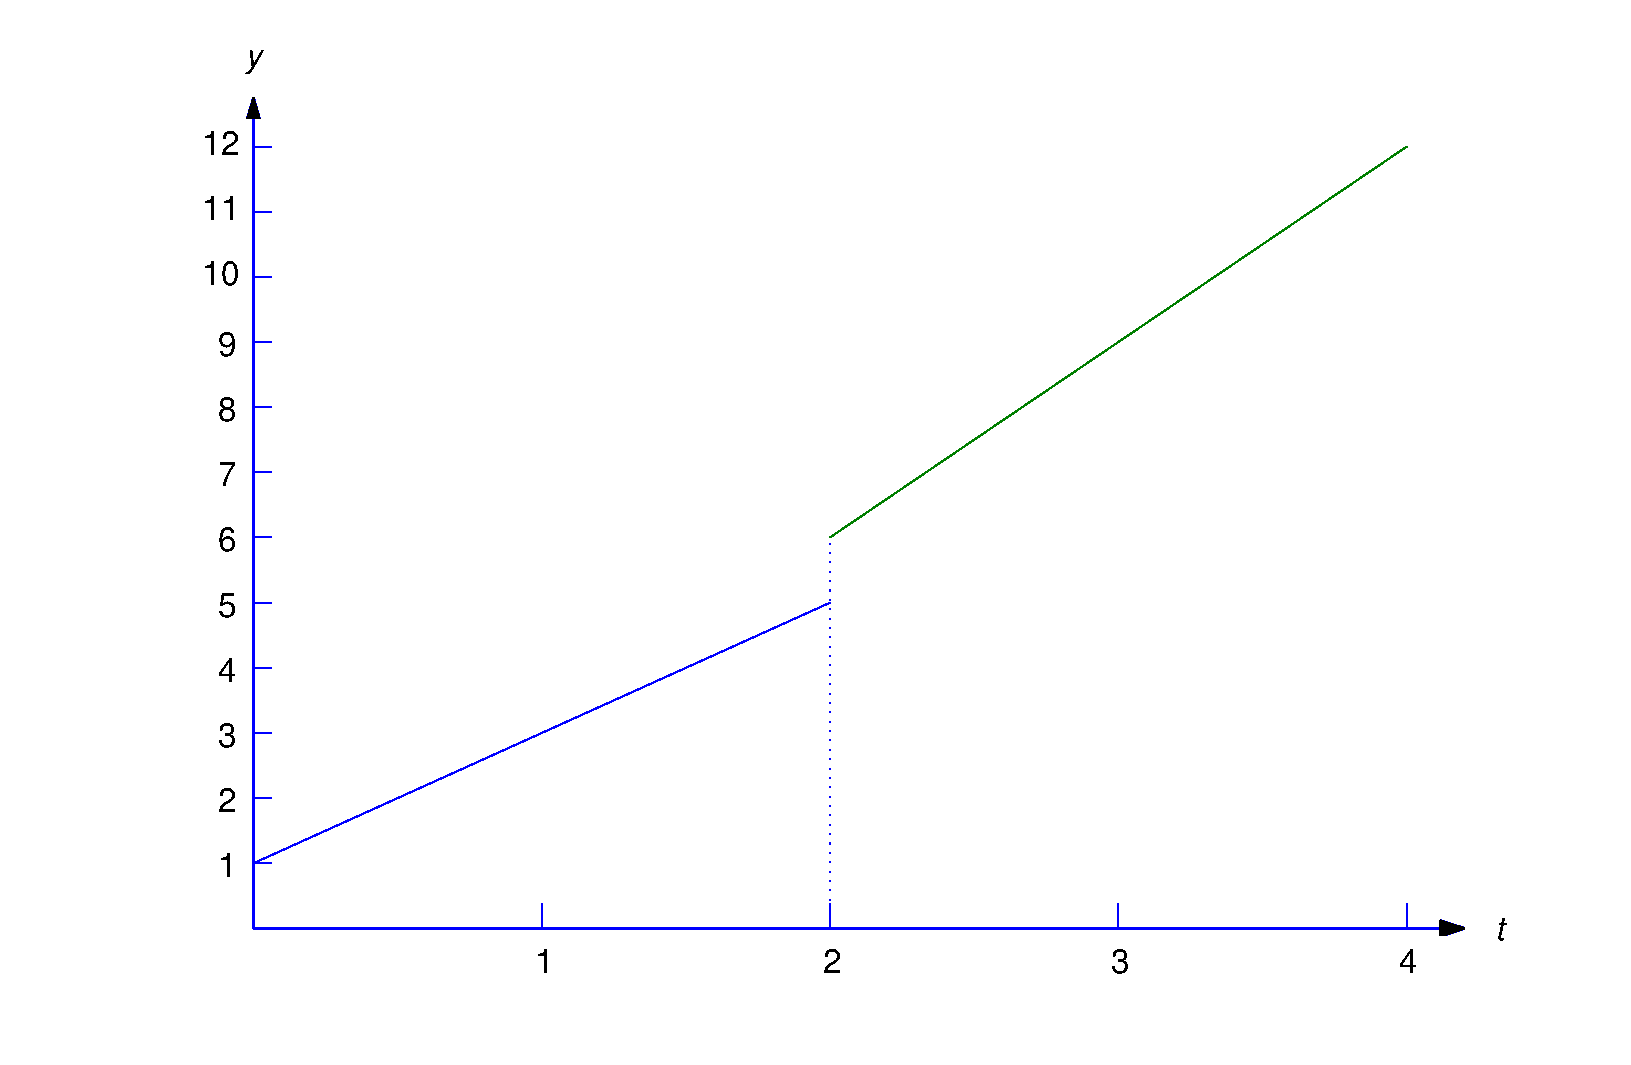
\includegraphics[bb=-78 148 689 643,width=5.67in,height=3.66in,keepaspectratio]{fig080401}}
\caption{The piecewise
 continuous function \eqref{eq:8.4.1}}
  \label{figure:8.4.1}
\end{minipage}
  \begin{minipage}[b]{0.5\linewidth}
    \centering
   \scalebox{.65}{
  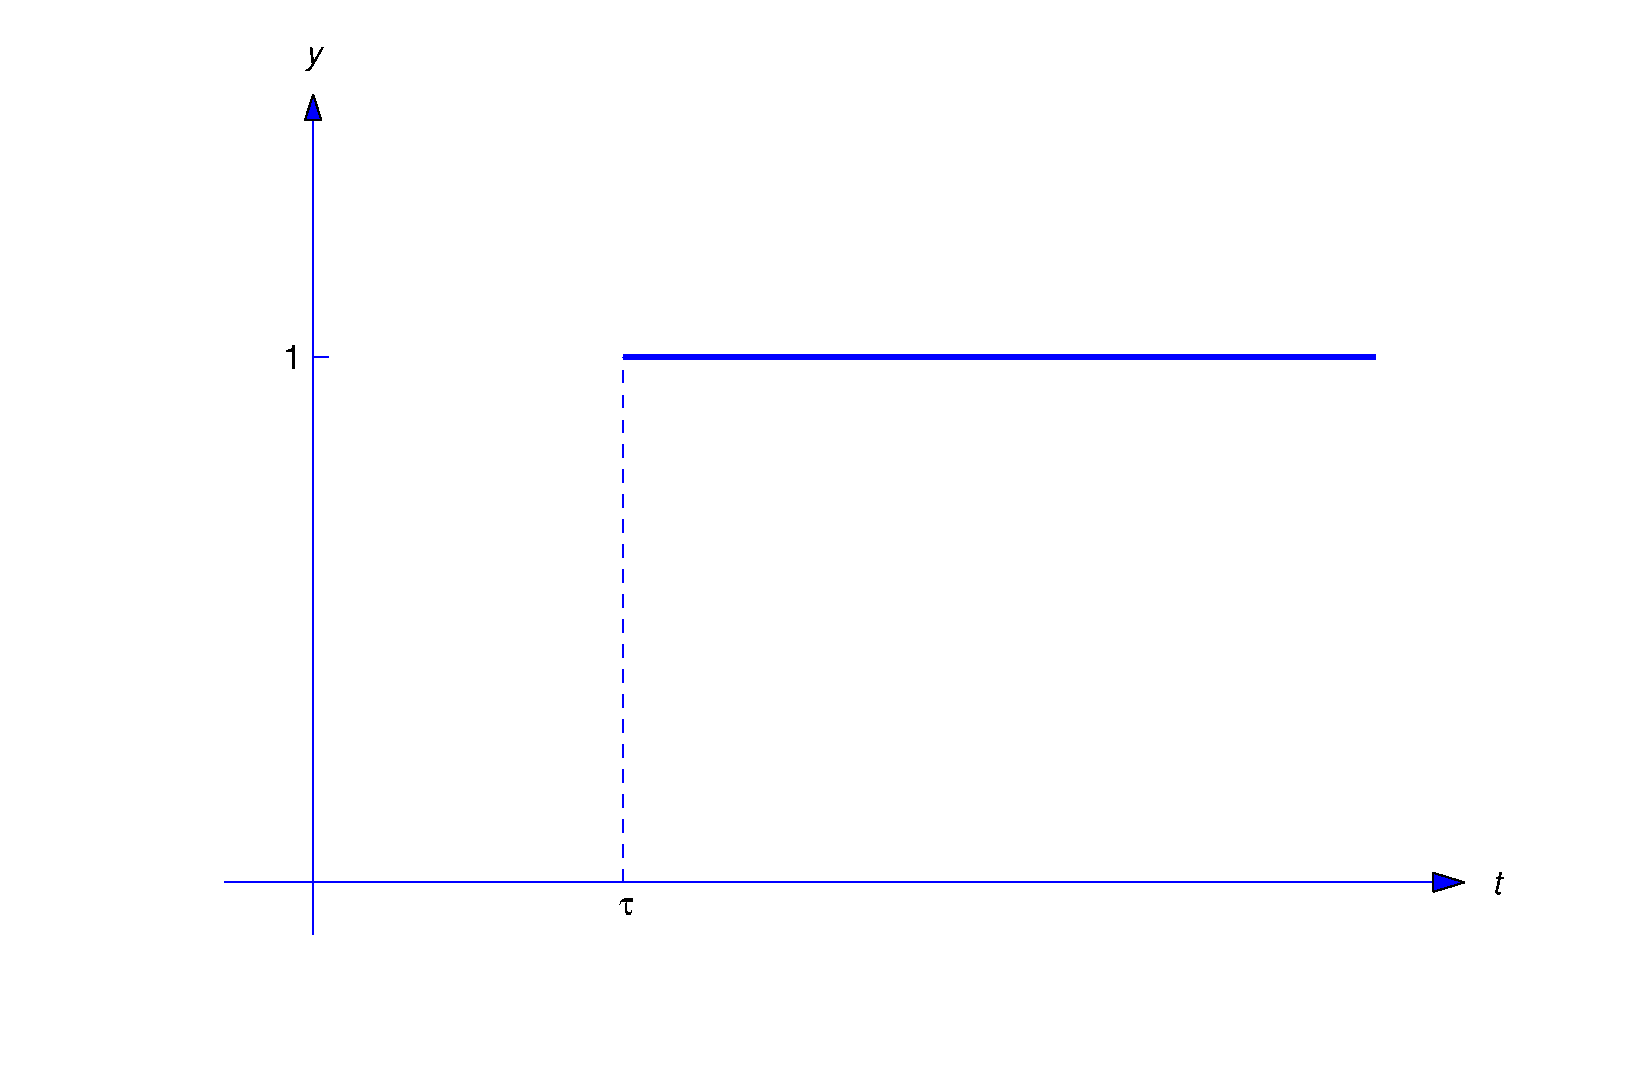
\includegraphics[bb=-78 148 689 643,width=5.67in,height=3.66in,keepaspectratio]{fig080402}}
\caption{ $y=u(t-\tau)$}
  \label{figure:8.4.2}
\end{minipage}
\end{figure}

\boxit{Laplace Transforms of Piecewise Continuous Functions}

\noindent
We'll now develop the method of Example~\ref{example:8.4.1} into a
systematic way to find the Laplace transform of a piecewise continuous
function. It is convenient to introduce the {\color{blue}\it unit step
function\/}, defined as
\begin{equation}\label{eq:8.4.4}
u(t)=\left\{\begin{array}{rl}
0,&t<0\\
1,&t\ge0.
\end{array}\right.
\end{equation}
Thus, $u(t)$ ``steps'' from the constant value $0$ to the constant
value $1$ at $t=0$. If we replace $t$ by
$t-\tau$ in \eqref{eq:8.4.4}, then
$$
u(t-\tau)=\left\{\begin{array}{rl}
0,&t<\tau,\\
1,&t\ge\tau
\end{array}\right.;
$$
that is, the step now occurs at $t=\tau$ (Figure~\ref{figure:8.4.2}).

The step function enables us to represent piecewise continuous
functions conveniently. For example, consider the function
\begin{equation}\label{eq:8.4.5}
f(t)=\left\{\begin{array}{rl}
f_0(t),&0\le t<t_1,\\[1\jot]
f_1(t),&t\ge t_1,
\end{array}\right.
\end{equation}
where we assume that $f_0$ and $f_1$ are defined on $[0,\infty)$, even
though they equal $f$ only on the indicated intervals. This assumption
enables us to rewrite \eqref{eq:8.4.5} as
\begin{equation}\label{eq:8.4.6}
f(t)=f_0(t)+u(t-t_1)\left(f_1(t)-f_0(t)\right).
\end{equation}
To verify this, note that if $t<t_1$ then $u(t-t_1)=0$ and
\eqref{eq:8.4.6}  becomes
$$
f(t)=f_0(t)+(0)\left(f_1(t)-f_0(t)\right)=f_0(t).
$$
If $t\ge t_1$ then $u(t-t_1)=1$ and  \eqref{eq:8.4.6} becomes
$$
f(t)=f_0(t)+(1)\left(f_1(t)-f_0(t)\right)=f_1(t).
$$

We need the next theorem to
 show how \eqref{eq:8.4.6} can be used to find ${\cal L}(f)$.

\begin{theorem}\color{blue}\label{thmtype:8.4.1}
Let $g$ be defined on $[0,\infty).$ Suppose   $\tau\ge0$ and ${\cal
L}\left(g(t+\tau)\right)$ exists for $s>s_0.$ Then ${\cal
L}\left(u(t-\tau)g(t)\right)$ exists for $s>s_0$, and
$$
{\cal L}(u(t-\tau)g(t))=e^{-s\tau}{\cal L}\left(g(t+\tau)\right).
$$
\end{theorem}

\proof By definition,
$$
{\cal L}\left(u(t-\tau)g(t)\right)=\int_0^\infty e^{-st} u(t-\tau)g(t)\,
dt.
$$
From this and the definition of $u(t-\tau)$,
$$
{\cal L}\left(u(t-\tau)g(t)\right)=\int_0^\tau
e^{-st}(0)\,dt+\int_{\tau}^\infty e^{-st}g(t)\,dt.
$$
The first integral on the right equals zero.  Introducing the new variable
of integration $x=t-\tau$ in the second integral yields
$$
{\cal L}\left(u(t-\tau)g(t)\right)=\int_0^\infty e^{-s(x+\tau)}g(x+\tau)\,dx
=e^{-s\tau}\int_0^\infty e^{-sx} g(x+\tau)\,dx.
$$
Changing the name of the variable of integration in the last integral
from $x$ to $t$ yields
$$
{\cal L}\left(u(t-\tau)g(t)\right)
=e^{-s\tau}\int_0^\infty e^{-st} g(t+\tau)\,dt=e^{-s\tau}{\cal
L}(g(t+\tau)).\bbox
$$

\begin{example}\label{example:8.4.2}\rm
 Find
$$
{\cal L}\left(u(t-1)(t^2+1)\right).
$$
\end{example}

\solution  Here $\tau=1$ and $g(t)=t^2+1$, so
$$
g(t+1)=(t+1)^2+1=t^2+2t+2.
$$
Since
$$
{\cal L}\left(g(t+1)\right)={2\over s^3}+{2\over s^2}+{2\over s},
$$
Theorem~\ref{thmtype:8.4.1} implies that
$${\cal L}\left(u(t-1)(t^2+1)\right)
=e^{-s}\left({2\over s^3}+{2\over s^2}+{2\over s}\right).
$$

\begin{example}\label{example:8.4.3}\rm
Use Theorem~\ref{thmtype:8.4.1} to find the Laplace transform of the
function
$$
f(t)=\left\{\begin{array}{cl} 2t+1,&0\le t<2,\\[1\jot] 3t,&t\ge2,
\end{array}\right.
$$
from Example~\ref{example:8.4.1}.
\end{example}

\solution
We first write $f$ in the form \eqref{eq:8.4.6} as
$$
f(t)=2t+1+u(t-2)(t-1).
$$
Therefore
\begin{eqnarray*}
{\cal L}(f)&=&{\cal L}(2t+1) +{\cal L}\left(u(t-2)(t-1)\right)\\
&=&{\cal L}(2t+1) +e^{-2s}{\cal L}(t+1)\quad\mbox{ (from
Theorem~\ref{thmtype:8.4.1}})\\
&=&{2\over s^2}+{1\over s}+e^{-2s}\left({1\over s^2}+{1\over s}\right),
\end{eqnarray*}
which is the result obtained in Example~\ref{example:8.4.1}.\bbox

Formula \eqref{eq:8.4.6} can be extended to more general piecewise continuous
functions. For example, we can write
$$
f(t)=\left\{\begin{array}{rl}
f_0(t),&0\le t<t_1,\\[1\jot]
f_1(t),&t_1\le t<t_2,\\[1\jot]
f_2(t),&t\ge t_2,
\end{array}\right.
$$
as
$$
f(t)=f_0(t)+u(t-t_1)\left(f_1(t)-f_0(t)\right)+
u(t-t_2)\left(f_2(t)-f_1(t)\right)
$$
if $f_0$, $f_1$, and $f_2$ are all defined on $[0,\infty)$.

\begin{example}\label{example:8.4.4}\rm
 Find the Laplace transform of
\begin{equation} \label{eq:8.4.7}
f(t)=\left\{\begin{array}{cl}
 1,&0\le t<2,\\[1\jot]
-2t+1,&2\le t<3,\\[1\jot]
 3t,&3\le t<5,\\[1\jot]
 t-1,&t\ge5
\end{array}\right.
\end{equation}
(Figure~\ref{figure:8.4.3}).
\end{example}

\begin{figure}[tbp]
  \centering\color{blue}
  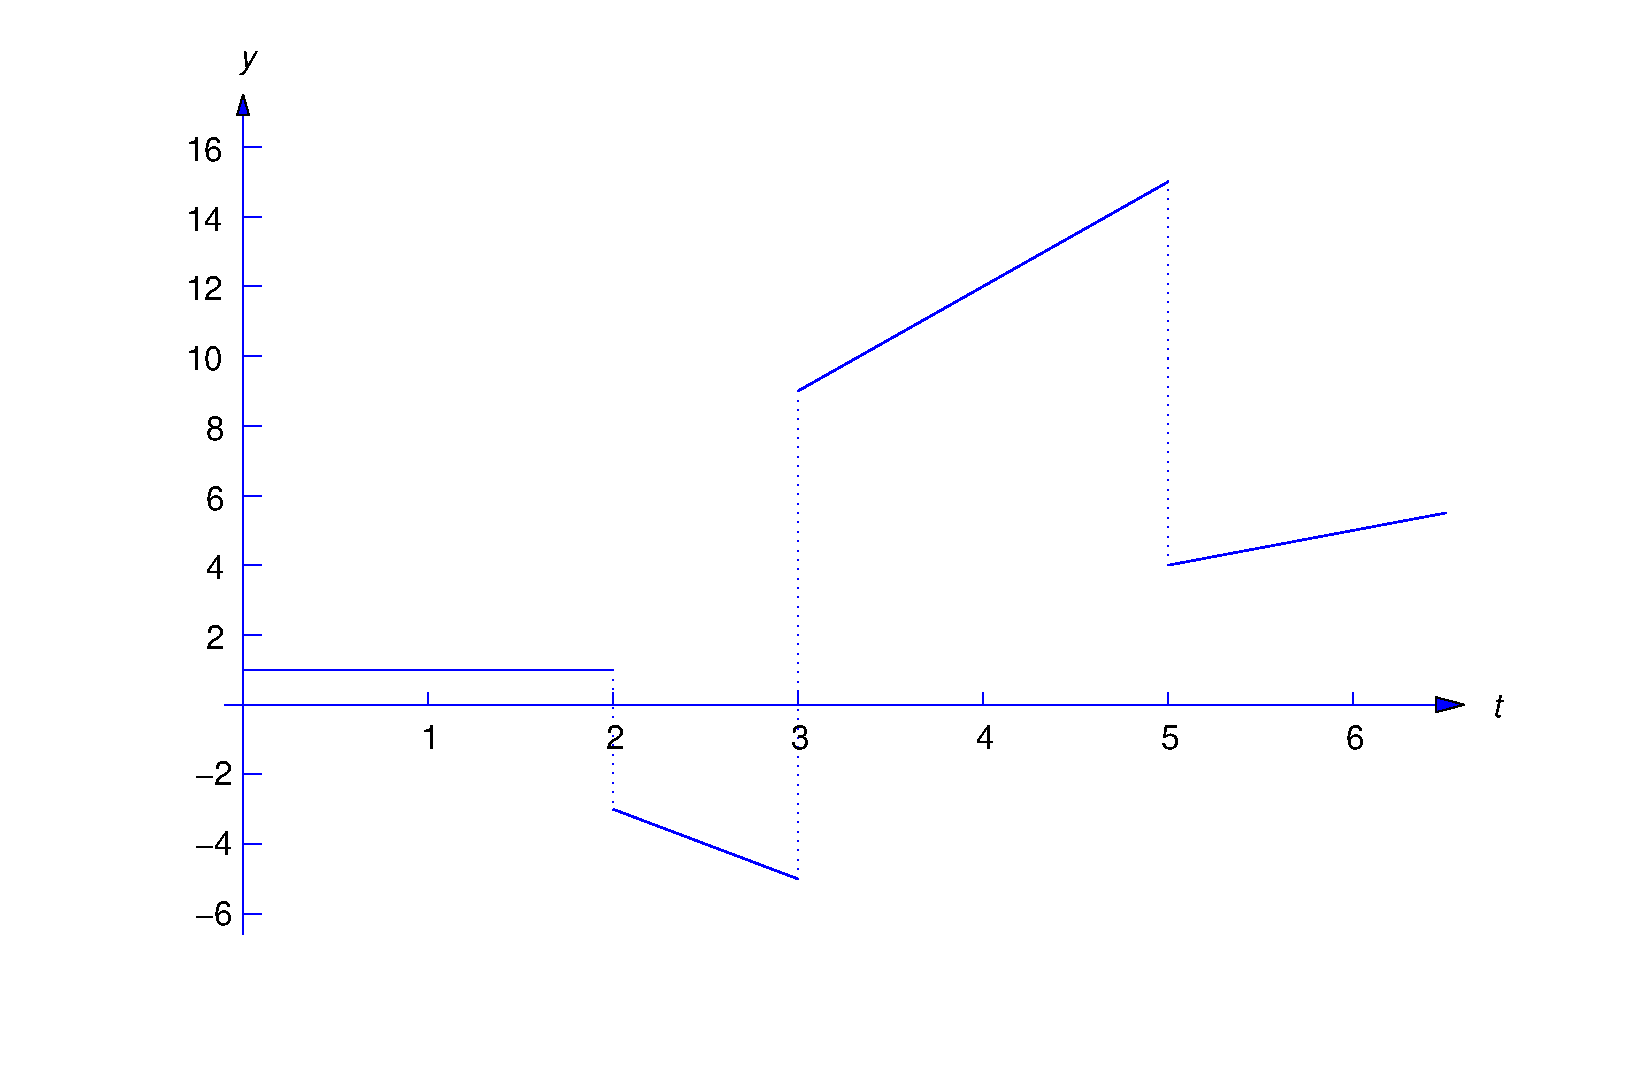
\includegraphics[bb=-78 148 689 643,width=5.67in,height=3.66in,keepaspectratio]{fig080403}
  \caption{The piecewise continuous function \eqref{eq:8.4.7}}
  \label{figure:8.4.3}
\end{figure}

\solution   In terms of step functions,
\begin{eqnarray*}
f(t)&=&1+u(t-2)(-2t+1-1)+u(t-3)(3t+2t-1)\\
&&+u(t-5)(t-1-3t),
\end{eqnarray*}
or
$$
f(t)=1-2u(t-2)t+u(t-3)(5t-1)-u(t-5)(2t+1).
$$
Now Theorem~\ref{thmtype:8.4.1} implies that
\begin{eqnarray*}
{\cal L}(f)&=&{\cal L}(1)-2e^{-2s}{\cal L}(t+2)+e^{-3s}{\cal
L}\left(5(t+3)-1\right)-e^{-5s}{\cal L}\left(2(t+5)+1\right)\\[1\jot]
&=&{\cal L}(1)-2e^{-2s}{\cal L}(t+2)+e^{-3s}{\cal
L}(5t+14)-e^{-5s}{\cal L}(2t+11)\\[1\jot]
&=&{1\over s}-2e^{-2s}\left({1\over s^2}+{2\over s}\right)+
e^{-3s}\left({5\over s^2}+{14\over s}\right)-e^{-5s}\left({2\over
s^2}+{11\over s}\right).\bbox
\end{eqnarray*}

 The trigonometric identities
\begin{eqnarray}
\sin (A+B)&=&\sin A\cos B+\cos A\sin B\label{eq:8.4.8}\\
\cos (A+B)&=&\cos A\cos B-\sin A\sin B\label{eq:8.4.9}
\end{eqnarray}
are useful in problems that involve shifting the arguments of
trigonometric functions. We'll use these identities in the next
example.

\begin{example}\label{example:8.4.5}\rm
 Find the Laplace transform of
\begin{equation} \label{eq:8.4.10}
f(t)=\left\{\begin{array}{cl}
\sin t,&0\le t<\dst{\pi\over 2},\\[2\jot]
\cos t-3\sin t,&\dst{\pi\over 2}\le t<\pi,\\[2\jot]
 3\cos t,&t\ge\pi
\end{array}\right.
\end{equation}
(Figure~\ref{figure:8.4.4}).
\end{example}

                 %
\begin{figure}[tbp]
  \centering\color{blue}
  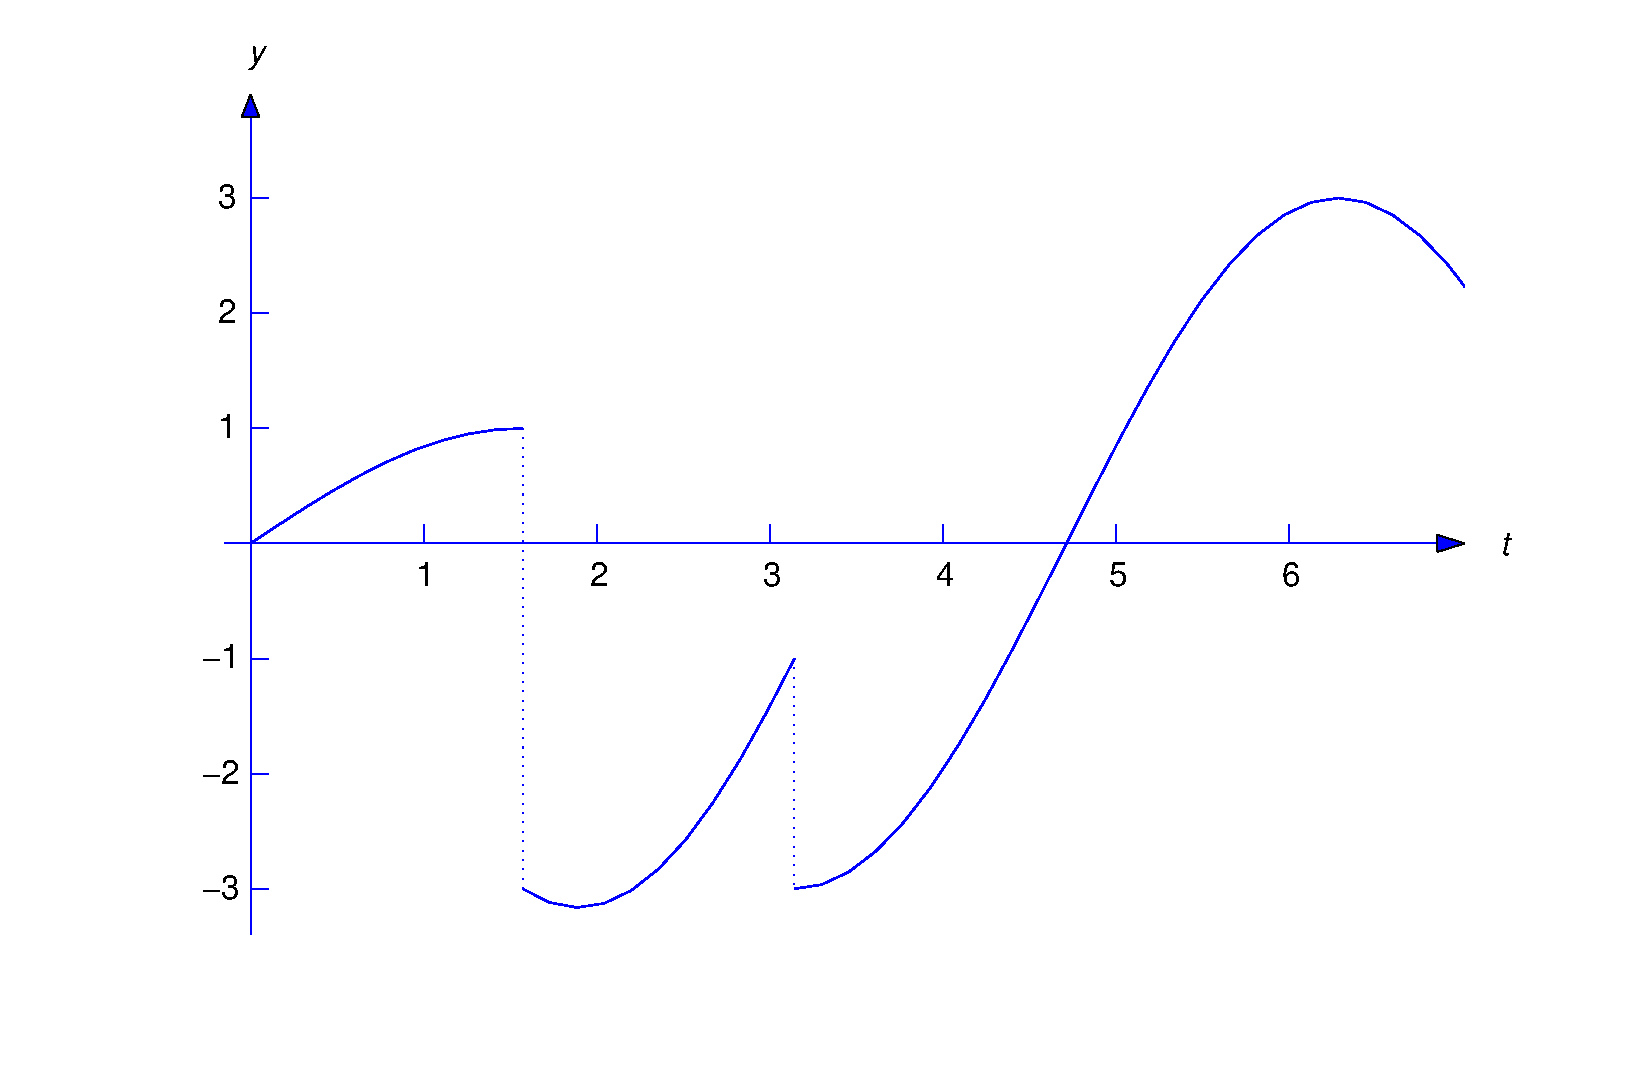
\includegraphics[bb=-78 148 689 643,width=5.67in,height=3.66in,keepaspectratio]{fig080404}
  \caption{The piecewise continuous function \eqref{eq:8.4.10}}
  \label{figure:8.4.4}
\end{figure}

 \solution In terms of step functions,
$$
f(t)=\sin t+u(t-\pi/2) (\cos t-4\sin t)+u(t-\pi) (2
\cos t+3\sin t).
$$
Now Theorem~\ref{thmtype:8.4.1} implies that
\begin{equation}\label{eq:8.4.11}
\begin{array}{ccl}
{\cal L}(f)&=&{\cal L}(\sin t)+e^{-{\pi\over 2}s}{\cal L}
\left(\cos\left(t+{\pi\over2}\right)-4\sin\left(t+{\pi\over2}\right)\right)\\
[1\jot]&&\qquad+e^{-\pi s}{\cal L}\left(2\cos(t+\pi)+3\sin(t+\pi)\right).
\end{array}
\end{equation}
Since
$$
\cos\left(t+{\pi\over 2}\right)-4\sin\left(t+{\pi\over
2}\right)=-\sin t-4\cos t
$$
and
$$
 2\cos (t+\pi)+3\sin (t+\pi)=-2\cos t-3\sin t,
$$
we see from \eqref{eq:8.4.11} that
\begin{eqnarray*}
{\cal L}(f)&=&{\cal L}(\sin t)-e^{-\pi s/2}{\cal L}(\sin t+4\cos t)
-e^{-\pi s}{\cal L}(2\cos t+3\sin t)\\[1\jot]
&=&{1\over s^2+1}-e^{-{\pi\over 2}s}\left({1+4s\over
s^2+1}\right)
-e^{-\pi s}\left({3+2s\over s^2+1}\right).\bbox
\end{eqnarray*}

\boxit{The Second Shifting Theorem}

\noindent
Replacing $g(t)$ by $g(t-\tau)$ in Theorem~\ref{thmtype:8.4.1}
yields the next theorem.

\begin{theorem}\color{blue}$[$Second Shifting
Theorem$]$\label{thmtype:8.4.2} If
 $\tau\ge0$ and ${\cal L}(g)$ exists for $s>s_0$
then  ${\cal L}\left(u(t-\tau)g(t-\tau)\right)$ exists for $s>s_0$ and
$$
{\cal L}(u(t-\tau)g(t-\tau))=e^{-s\tau}{\cal L}(g(t)),
$$
or, equivalently,
\begin{equation}\label{eq:8.4.12}
\mbox{if } g(t)\leftrightarrow G(s),\mbox{ then
}u(t-\tau)g(t-\tau)\leftrightarrow e^{-s\tau}G(s).
\end{equation}
\end{theorem}

\color{blue}
\remark{ Recall that the First Shifting Theorem
(Theorem~\ref{thmtype:8.1.3} states that multiplying a function  by
$e^{at}$ corresponds to shifting the argument of its transform by $a$
units. Theorem~\ref{thmtype:8.4.2} states that multiplying a Laplace
transform by the exponential $e^{-\tau s}$ corresponds to shifting the
argument of the inverse transform by $\tau$ units.}
\color{black}

\begin{example}\label{example:8.4.6}\rm
 Use \eqref{eq:8.4.12} to find
$$
{\cal L}^{-1}\left(e^{-2s}\over s^2\right).
$$
\end{example}

\solution  To apply \eqref{eq:8.4.12} we let
$\tau=2$ and $G(s)=1/s^2$. Then $g(t)=t$ and \eqref{eq:8.4.12} implies that
$$
{\cal L}^{-1}\left(e^{-2s}\over s^2\right)=u(t-2)(t-2).\bbox
$$

\begin{example}\label{example:8.4.7}\rm
 Find the inverse Laplace transform $h$ of
$$
H(s)={1\over s^2}-e^{-s}\left({1\over s^2}+{2\over s}\right)+
e^{-4s}\left({4\over s^3}+{1\over s}\right),
$$
and find distinct formulas for $h$ on appropriate intervals.
\end{example}

\solution  Let
$$
G_0(s)={1\over s^2},\quad G_1(s)={1\over s^2}+{2\over s},\quad
G_2(s)={4\over s^3}+{1\over s}.
$$
Then
$$
g_0(t)=t,\; g_1(t)=t+2,\; g_2(t)=2t^2+1.
$$
Hence, \eqref{eq:8.4.12} and the linearity of ${\cal L}^{-1}$ imply that
\begin{eqnarray*}
h(t)&=&{\cal L}^{-1}\left(G_0(s)\right)-{\cal
L}^{-1}\left(e^{-s}G_1(s)\right)+{\cal
L}^{-1}\left(e^{-4s}G_2(s)\right)\\[1\jot]
&=&t-u(t-1)\left[(t-1)+2\right]+u(t-4)\left[2(t-4)^2+1\right]\\[1\jot]
&=&t-u(t-1)(t+1)+u(t-4)(2t^2-16t+33),
\end{eqnarray*}
which can also be written as
$$
h(t)=\left\{\begin{array}{cl}
 t,&0\le t<1,\\[1\jot]
-1,&1\le t<4,\\[1\jot]
2t^2-16t+32,&t\ge4.
\end{array}\right.\bbox
$$

\begin{example}\label{example:8.4.8}\rm
 Find the inverse transform of
$$
H(s)={2s\over s^2+4}-e^{-{\pi\over 2}s} {3s+1\over s^2+9}+e^{-\pi
s}{s+1\over s^2+6s+10}.
$$
\end{example}

\solution  Let
$$
G_0(s)={2s\over s^2+4},\quad G_1(s)=-{(3s+1)\over s^2+9},
$$
and
$$
G_2(s)={s+1\over s^2+6s+10}={(s+3)-2\over (s+3)^2+1}.
$$
Then
$$
g_0(t)=2\cos 2t,\quad g_1(t)=-3\cos 3t-{1\over 3}\sin 3t,
$$
and
$$
g_2(t)=e^{-3t}(\cos t-2\sin t).
$$
Therefore \eqref{eq:8.4.12} and the linearity of ${\cal L}^{-1}$
imply that
\begin{eqnarray*}
h(t)&=&2\cos 2t-u(t-\pi/2)\left[3\cos
3(t-\pi/2)+{1\over 3}\sin 3\left(t-{\pi\over
2}\right)\right]\\[2\jot]
&&+u(t-\pi)e^{-3(t-\pi)}\left[\cos (t-\pi)-2\sin (t-\pi)\right].
\end{eqnarray*}
Using the trigonometric identities  \eqref{eq:8.4.8} and
\eqref{eq:8.4.9}, we can rewrite this as
\begin{equation} \label{eq:8.4.13}
\begin{array}{rcl}
h(t)&=&2\cos 2t+u(t-\pi/2)\left(3\sin 3t-
{1\over 3}\cos 3t\right)\\[2\jot]
&&-u(t-\pi)e^{-3(t-\pi)} (\cos t-2\sin t)
\end{array}
\end{equation}
(Figure~\ref{figure:8.4.5}).

\begin{figure}[H]
  \centering\color{blue}
  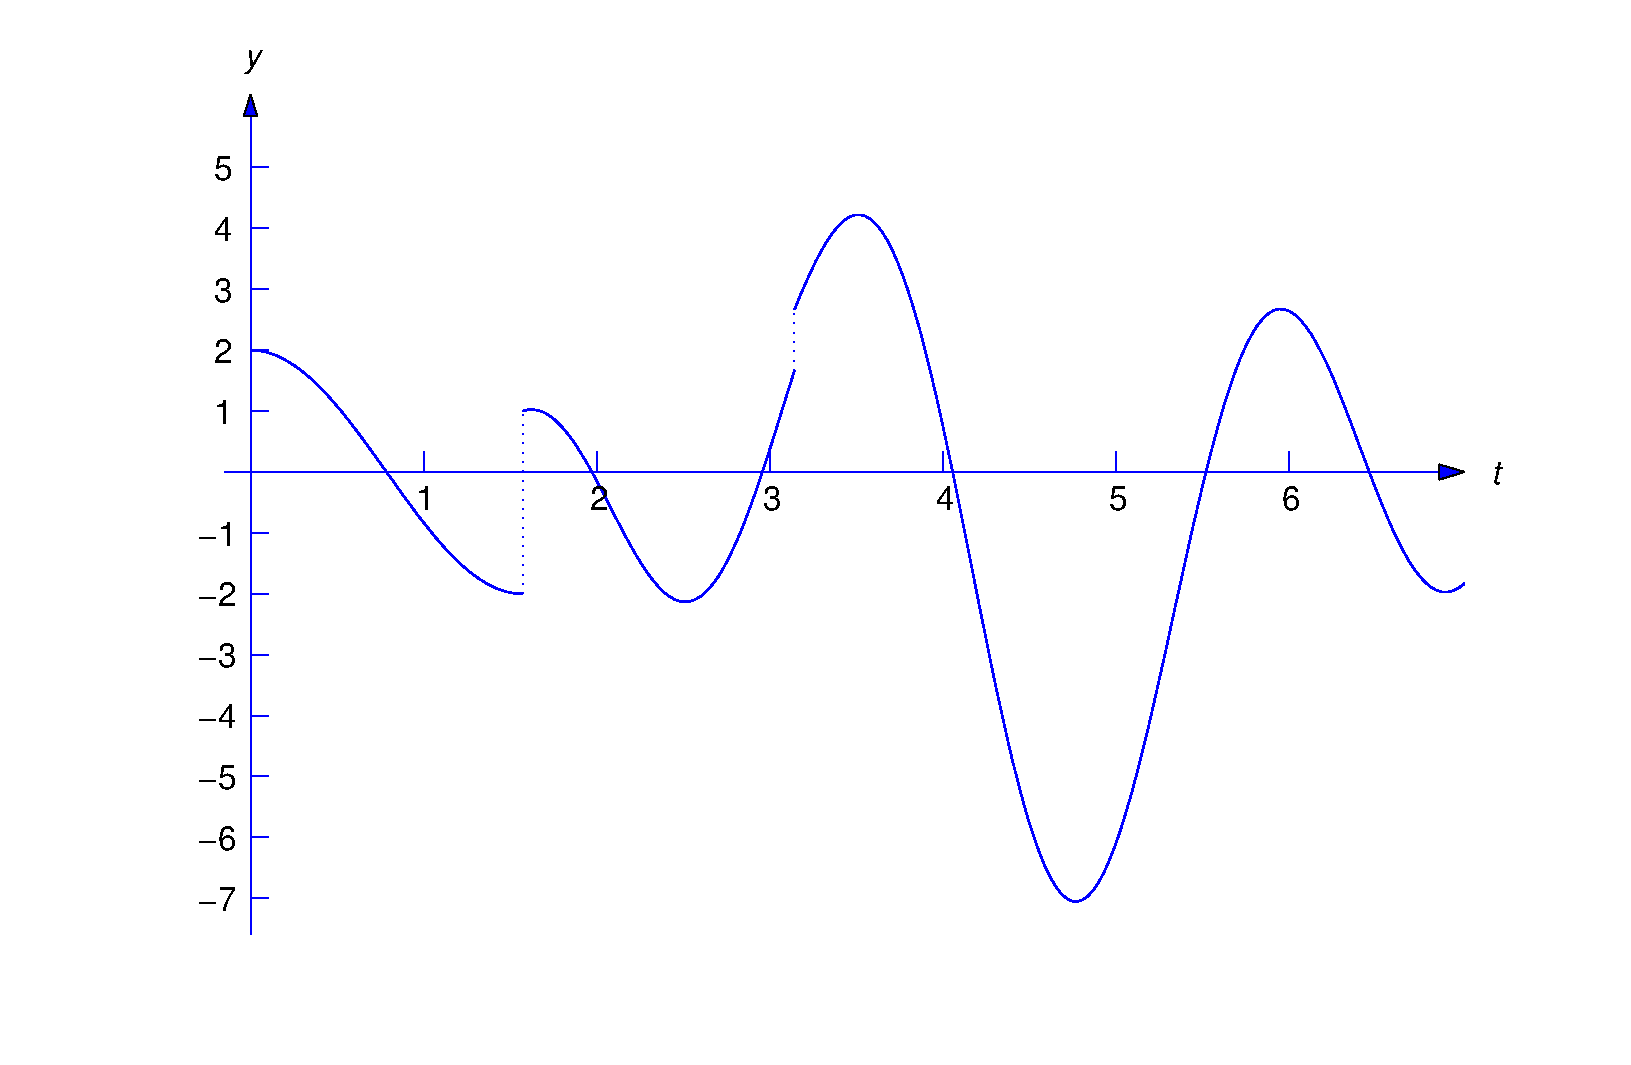
\includegraphics[bb=-78 148 689 643,width=5.67in,height=3.66in,keepaspectratio]{fig080405}
  \caption{ The piecewise continuous function
\eqref{eq:8.4.13}}
  \label{figure:8.4.5}
\end{figure}

 \exercises
In Exercises~\ref{exer:8.4.1}--\ref{exer:8.4.6} find the Laplace transform by
the method of Example~\ref{example:8.4.1}. Then express the given function
$f$ in terms of unit step functions as in Eqn.~\eqref{eq:8.4.6}, and use
Theorem~\ref{thmtype:8.4.1} to find ${\cal L}(f)$.
Where indicated by \CGex, graph $f$.
\begin{exerciselist}

\begin{tabular}[t]{@{}p{168pt}@{}p{168pt}}
\item\label{exer:8.4.1} $\dst{f(t)=\left\{\begin{array}{cl} 1,&0
\le t<4,\\[2\jot] t,&t\ge4.\end{array}\right.}$&
\item\label{exer:8.4.2} $\dst{f(t)=\left\{\begin{array}{cl} t,&0
\le t<1,\\[2\jot] 1,&t\ge1.\end{array}\right.}$
\end{tabular}

\begin{tabular}[t]{@{}p{168pt}@{}p{168pt}}
\item\label{exer:8.4.3} \CGex $\dst{f(t)=\left\{\begin{array}{cl} 2t-1,&
0\le t<2,\\[2\jot]  t,&t\ge2.\end{array}\right.}$&
\item\label{exer:8.4.4} \CGex $\dst{f(t)=\left\{\begin{array}{cl}1,
&0\le t<1,\\[2\jot] t+2,&t\ge1.\end{array}\right.}$
\end{tabular}

\begin{tabular}[t]{@{}p{168pt}@{}p{168pt}}
\item\label{exer:8.4.5}$\dst{f(t)=\left\{\begin{array}{cl} t-1,& 0\le
t<2,\\[2\jot] 4,&t\ge2.\end{array}\right.}$&
\item\label{exer:8.4.6} $\dst{f(t)=\left\{\begin{array}{cl} t^2,& 0\le
t<1,\\[2\jot] 0,&t\ge1.\end{array}\right.}$
\end{tabular}

\exercisetext{In Exercises~\ref{exer:8.4.7}--\ref{exer:8.4.18} express the
given function $f$ in terms of unit step functions
 and use Theorem~\ref{thmtype:8.4.1} to find ${\cal
L}(f)$.
Where indicated by \CGex, graph $f$.}

\begin{tabular}[t]{@{}p{168pt}@{}p{168pt}}
\item\label{exer:8.4.7}$\dst{f(t)=\left\{\begin{array}{cl} 0, &0\le
t<2,\\[2\jot] t^2+3t,&t\ge2.\end{array}\right.}$&
\item\label{exer:8.4.8} $\dst{f(t)=\left\{\begin{array}{cl} t^2+2, &0\le
t<1,\\[2\jot] t,&t\ge1.\end{array}\right.}$
\end{tabular}

\begin{tabular}[t]{@{}p{168pt}@{}p{168pt}}
\item\label{exer:8.4.9} $\dst{f(t)=\left\{\begin{array}{cl} te^t,& 0\le t
<1,\\[2\jot] e^t,&t\ge1.\end{array}\right.}$&
\item\label{exer:8.4.10} $\dst{f(t)=\left\{\begin{array}{cl}
e^{\phantom{2}-t}, &0\le t<1,\\[2\jot]
e^{-2t},&t\ge1.\end{array}\right.}$
\end{tabular}

\begin{tabular}[t]{@{}p{168pt}@{}p{168pt}}
\item\label{exer:8.4.11} $\dst{f(t)=\left\{\begin{array}{cl} -t,&0 \le
t<2,\\[2\jot] t-4,&2\le t<3,\\[2\jot] 1,&t\ge3.
\end{array}\right.}$&
\item\label{exer:8.4.12} $\dst{f(t)=\left\{\begin{array}{cl} 0,&0 \le
t<1,\\[2\jot] t,&1\le t<2,\\[2\jot] 0,&t\ge2.\end{array}\right.}$
\end{tabular}

\begin{tabular}[t]{@{}p{168pt}@{}p{168pt}}
\item\label{exer:8.4.13} $\dst{f(t)=\left\{\begin{array}{cl} t,&0 \le
t<1,\\[2\jot] t^2,&1\le t<2,\\[2\jot] 0,&t\ge2. \end{array}\right.}$&
\item\label{exer:8.4.14} $\dst{f(t)=\left\{\begin{array}{cl} t,&0\le
t<1,\\[2\jot] 2-t,&1\le t<2,\\[2\jot] 6,&t > 2. \end{array}\right.}$
\end{tabular}

\item\label{exer:8.4.15} \CGex $\dst{f(t)=\left\{\begin{array}{cl}
\phantom{2}
\sin t,&0\le t<\dst{\pi\over 2},\\[2\jot] 2\sin t,&
\dst{\pi\over 2}\le t<\pi,\\[2\jot]\phantom{2}\cos t,
&t\ge\pi.\end{array}\right.}$

\item\label{exer:8.4.16} \CGex
$f(t)=\dst{\left\{\begin{array}{cl}\phantom{-} 2,&0\le
t<1,\\[2\jot]-2t+2,&1\le t<3,\\[2\jot]\phantom{-}3t,&t\ge
3.\end{array}\right.}$

\item\label{exer:8.4.17}  \CGex
$f(t)=\dst{\left\{\begin{array}{cl}3,&0\le t<2,\\[2\jot]3t+2,&2\le
t<4,\\[2\jot]4t,&t\ge
4.\end{array}\right.}$

\item\label{exer:8.4.18}  \CGex
$\dst{f(t)=\left\{\begin{array}{ll}(t+1)^2,&0\le t<1,
\\[2\jot](t+2)^2,&t\ge1.\end{array}\right.}$

\exercisetext{In Exercises~\ref{exer:8.4.19}--\ref{exer:8.4.28} use
Theorem~\ref{thmtype:8.4.2} to express the inverse transforms in terms of
step functions, and then find distinct formulas the for inverse
transforms on the appropriate intervals, as in
Example~\ref{example:8.4.7}.
Where indicated by \CGex, graph the inverse transform.}

\begin{tabular}[t]{@{}p{168pt}@{}p{112pt}@{}p{68pt}}
\item\label{exer:8.4.19} $\dst{H(s)={e^{-2s}\over s-2}}$&
\item\label{exer:8.4.20} $\dst{H(s)={e^{-s}\over s(s+1)}}$
\end{tabular}

\item\label{exer:8.4.21} \CGex $\dst{H(s)={e^{-s}\over s^3}+
{e^{-2s}\over s^2}}$

\item\label{exer:8.4.22} \CGex $\dst{H(s)=\left({2\over s}+{1\over s^2}\right)
+e^{-s}\left({3\over s}-{1\over s^2}\right)+e^{-3s}\left({1\over
s}+{1\over s^2}\right)}$

\item\label{exer:8.4.23} $\dst{H(s)=\left({5\over s}-{1\over s^2}\right)
+e^{-3s}\left({6\over s}+{7\over s^2}\right)+{3e^{-6s}\over s^3}}$

\item\label{exer:8.4.24} $\dst{H(s)={e^{-\pi s} (1-2s)\over s^2+4s+5}}$

\item\label{exer:8.4.25} \CGex $\dst{H(s)=\left({1\over s}-{s\over
s^2+1}\right)+e^{-{\pi\over 2}s}\left({3s-1\over s^2+1}\right)}$

\item\label{exer:8.4.26} $\dst{H(s)=
e^{-2s}\left[{3(s-3)\over(s+1)(s-2)}-{s+1\over(s-1)(s-2)}\right]}$

\item\label{exer:8.4.27} $\dst{H(s)={1\over s}+{1\over
s^2}+e^{-s}\left({3\over s}+{2\over s^2}\right) +e^{-3s}\left({4\over
s}+{3\over s^2}\right)}$

\item\label{exer:8.4.28} $\dst{H(s)={1\over s}-{2\over
s^3}+e^{-2s}\left({3\over s}-{1\over s^3}\right) +{e^{-4s}\over s^2}}$

\item\label{exer:8.4.29} Find ${\cal L}\left(u(t-\tau)\right)$.

\item\label{exer:8.4.30}
Let $\{t_m\}_{m=0}^\infty$ be a sequence of points such that $t_0=0$,
$t_{m+1}>t_m$, and $\lim_{m\to\infty}t_m=\infty$. For each nonnegative
integer $m$, let $f_m$ be continuous on $[t_m,\infty)$, and let $f$ be
defined on $[0,\infty)$ by
$$
f(t)=f_m(t),\,t_m\le t<t_{m+1}\quad (m=0,1,\dots).
$$
Show that $f$ is piecewise continuous on $[0,\infty)$  and
that it has the step function representation
$$
f(t)=f_0(t)+\sum_{m=1}^\infty u(t-t_m)\left(f_m(t)-f_{m-1}(t)\right),\,
0\le t<\infty.
$$
How do we know that the series on the right converges for all $t$
in $[0,\infty)$?

\item\label{exer:8.4.31}
In addition to the assumptions of Exercise~\ref{exer:8.4.30},
assume that
$$
|f_m(t)|\le Me^{s_0t},\,t\ge t_m,\,m=0,1,\dots,
\eqno{\rm (A)}
$$
and that the series
$$
\sum_{m=0}^\infty e^{-\rho t_m}
\eqno{\rm (B)}
$$
converges for some $\rho>0$. Using the  steps listed below, show
that
${\cal L}(f)$ is defined for $s>s_0$  and
$$
{\cal L}(f)={\cal L}(f_0)+\sum_{m=1}^\infty e^{-st_m}{\cal L}(g_m)
\eqno{\rm (C)}
$$
for $s>s_0+\rho$,
where
$$
g_m(t)=f_m(t+t_m)-f_{m-1}(t+t_m).
$$

\begin{alist} % (a)
\item
Use (A) and Theorem~8.1.6 to show that
$$
{\cal
L}(f)=\sum_{m=0}^\infty\int_{t_m}^{t_{m+1}}e^{-st}f_m(t)\,dt
\eqno{\rm (D)}
$$
is defined for $s>s_0$.
\item % (b)
Show that  (D) can be rewritten as
$$
{\cal L}(f)=\sum_{m=0}^\infty\left(\int_{t_m}^\infty e^{-st}f_m(t)\,dt
-\int_{t_{m+1}}^\infty e^{-st}f_m(t)\,dt\right).
\eqno{\rm (E)}
$$
\item % (c)
Use  (A), the assumed convergence of  (B), and the
comparison test  to show that the series
$$
\sum_{m=0}^\infty\int_{t_m}^\infty e^{-st}f_m(t)\,dt\mbox{\quad and \quad}
\sum_{m=0}^\infty\int_{t_{m+1}}^\infty e^{-st}f_m(t)\,dt
$$
both converge (absolutely) if $s>s_0+\rho$.
\item % (d)
Show that  (E) can be rewritten as
 $$
{\cal L}(f)={\cal L}(f_0)+\sum_{m=1}^\infty\int_{t_m}^\infty e^{-st}
\left(f_m(t)-f_{m-1}(t)\right)\,dt
$$
if $s>s_0+\rho$.
\item % (e)
Complete the proof of  (C).
\end{alist}

\item\label{exer:8.4.32} Suppose $\{t_m\}_{m=0}^\infty$ and
$\{f_m\}_{m=0}^\infty$ satisfy the assumptions of
Exercises~\ref{exer:8.4.30} and \ref{exer:8.4.31}, and
there's a positive constant $K$ such that $t_m\ge Km$ for $m$
sufficiently large. Show that the series  (B) of
Exercise~\ref{exer:8.4.31} converges for any $\rho>0$, and conclude from
this that  (C) of Exercise~\ref{exer:8.4.31} holds for $s>s_0$.

\exercisetext{In Exercises~\ref{exer:8.4.33}--\ref{exer:8.4.36} find the step
function representation of $f$ and use the result of
Exercise~\ref{exer:8.4.32} to find ${\cal L}(f)$. \hint{You will need
formulas related to the formula for the sum of a geometric series.}}

\item\label{exer:8.4.33}
$f(t)=m+1,\,m\le t<m+1\; (m=0,1,2,\dots)$

\item\label{exer:8.4.34}
$f(t)=(-1)^m,\,m\le t<m+1\; (m=0,1,2,\dots)$

\item\label{exer:8.4.35}
$f(t)=(m+1)^2,\,m\le t<m+1\; (m=0,1,2,\dots)$

\item\label{exer:8.4.36}
$f(t)=(-1)^mm,\,m\le t<m+1\; (m=0,1,2,\dots)$
\end{exerciselist}
